\chapter{Methodology}
\label{chap:2}
\ChapterPageStuff{2}

\section{Preamble}
In this chapter the methodology to create and implement a loggign mechanism to do system utilisation analysis on software system will be discussed. In \Cref{sec:EventLogging} provided the needed literature to create a loggign mechanism in \Cref{sec:Ch3_LoggingMechanism}.

\section{Logging mechanism}\label{sec:Ch3_LoggingMechanism}

\subsection{Logging points}
Loggign point are essential data that describes the event's key features when creating a log as discussed in \Cref{sec:Ch1_LoggignPoints}.

\begin{table}[!htb]
	\centering
	\small
	\caption[Loggign points]
	{\textit{PHP loggign mechanism}}
	\label{tbl:PHP_LoggignMechanism}
	\begin{tabularx}{\textwidth}{|c|c|X|}
		\hline \textbf{Identification} & \textbf{Criteria} & \textbf{Description} \\
        \hline \textit{lma\_ID} & Activity ID & The activity identification is a incremental number of the event that is logged.\\
        \hline \textit{lma\_Time} & Activity timestamp & This is the time which the event took place.\\
        \hline \textit{lma\_d\_ID} & Dashboard ID & Foreign reference key to the  \\
		\hline
	\end{tabularx}
\end{table}

\begin{figure}[!htb] % An h :here, t: top, b: bottom.
	\centering % cent the figure
	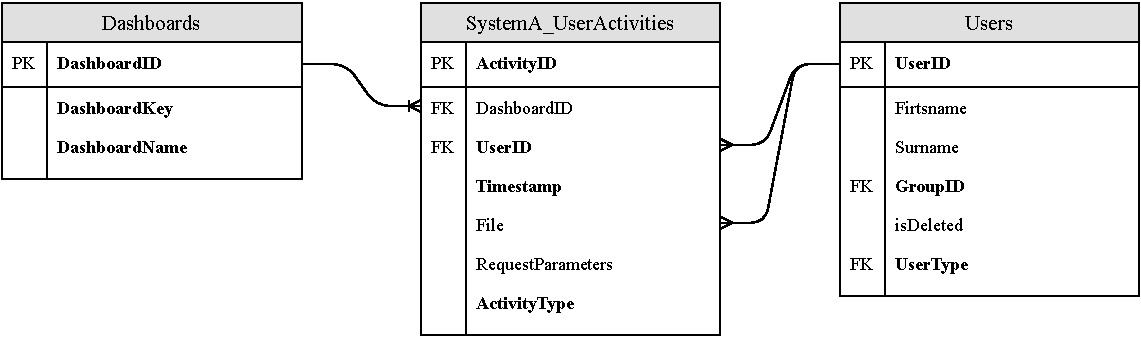
\includegraphics[width=0.9\textwidth]{Images/Chapter2/SystemA_ERD_Basic/SystemA_ERD_Basic.pdf}
	\caption[System A user activity ERD]
	{\textit{System A user activity ERD}} \label{fig:SystemA_Basic_ERD}
\end{figure}

\begin{figure}[!htb] % An h :here, t: top, b: bottom.
	\centering % cent the figure
	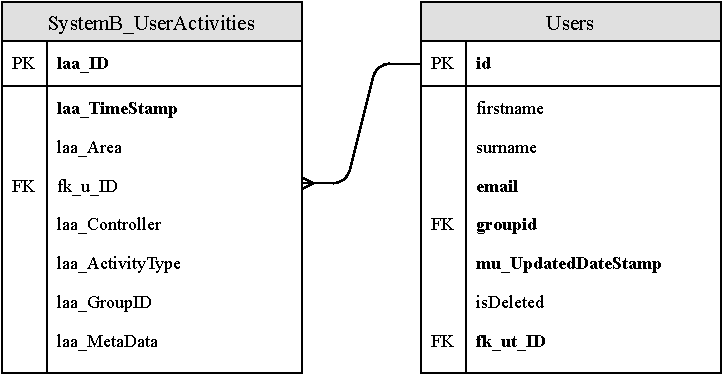
\includegraphics[width=0.9\textwidth]{Images/Chapter2/SystemB_ERD_Basic/SystemB_ERD_Basic.pdf}
	\caption[System B user activity ERD]
	{\textit{System B user activity ERD}} \label{fig:SystemB_Basic_ERD}
\end{figure}

\subsection{Logging mechanism}

\section{System utilisation analysis}

\section{Integration}
In this section the integration of the utilisation analysis and logging mechanism will be discussed.

\section{Conclusion}
Conclude the chapter about the development of the logging mechanism and utilisation analysis.